\documentclass[12pt,a4paper]{article}
\usepackage[T1]{fontenc}
\usepackage[english]{babel}
\usepackage{microtype}
\usepackage{amsmath,amsfonts,amssymb,amsthm}
\usepackage{graphicx}
\usepackage{geometry}
\usepackage{hyperref}
\usepackage{fancyhdr}
\usepackage{enumitem}
\usepackage{float}
\usepackage{mathtools}
\usepackage{csquotes}
\usepackage{xcolor}

\geometry{left=3cm,right=3cm,top=3cm,bottom=3cm,headheight=15pt}
\addtolength{\topmargin}{-2.5pt}

\pagestyle{fancy}
\fancyhf{}
\fancyhead[L]{MATH 477 Applied Finite Element Analysis}
\fancyhead[R]{Homework Report \#3}
\fancyfoot[C]{\thepage}
\renewcommand{\headrulewidth}{0.4pt}
\renewcommand{\footrulewidth}{0.4pt}

\begin{document}

% ========= Title =========
\begin{titlepage}
  \centering
  \vspace*{0.5cm}
  {\Large\bfseries MATH 477 Applied Finite Element Analysis\par}
  \vspace{1cm}
  {\large Homework Report \#3\par}
  \vspace{0.5cm}
  {October 19, 2025\par}
  \vspace{0.7cm}
  
\includegraphics[width=0.3\textwidth]{NU-logo.png}\\[0.3cm]
  
\includegraphics[width=0.18\textwidth]{sosah-logo.png}\\[0.3cm]
  \vspace{0.3cm}
  Submitted for {\bf MATH 477 Applied Finite Element Analysis}, Department of Mathematics,\\
  School of Sciences and Humanities, Nazarbayev University

  \vspace{0.6cm}
  {\large Student Name:\par}
  \begin{itemize}[leftmargin=6cm]
    \item Alizhan Zhapan
  \end{itemize}
  \vspace{0.5cm}
  \flushleft{
    Subject Area {\bf Applied Finite Element Analysis}\\
    Description {\bf Homework Report}\\
    Course Instructor {\bf Dongming Wei}\\[0.5cm]
    {\footnotesize By turning in this report I confirm that I have read the Academic Integrity Policy and that any borrowed material is cited.}
  }
\end{titlepage}

% ========= Problems =========
\newpage
\section*{Homework 3 Due Oct 6 2025}
\setcounter{section}{0}

\subsection*{Problem 1}
Study the boundary value model
\[
-\,u''(x)+u(x)=1,\qquad 0<x<1,\qquad u(0)=0,\; u'(1)=0.
\]
\begin{enumerate}[label=(\alph*)]
  \item Obtain the exact field by the Laplace transform route.
  \item Use three nodes $x_1=0$, $x_2=\tfrac12$, $x_3=1$ and a single quadratic interpolation. Write
  \(
  u_{\mathrm{app}}(x)=\alpha x^{2}+\beta x+\gamma
  \)
  and match $u_{\mathrm{app}}(x_i)=u(x_i)$ for $i=1,2,3$. Express the interpolant as
  \(
  u_{\mathrm{app}}(x)=\sum_{i=1}^{3}\varphi_i(x)\, \upsilon_i
  \)
  with nodal values $\upsilon_1=u(0)$, $\upsilon_2=u(\tfrac12)$, $\upsilon_3=u(1)$. Form the Galerkin equations and write the $3\times3$ matrix for the unknowns $\upsilon_2$ and $\upsilon_3$ after imposing $u(0)=0$ and the natural condition at $x=1$.
  \item Plot the exact field and the quadratic finite element field and comment on their difference.
\end{enumerate}

\subsection*{Problem 2}
Consider
\[
-\,u''(x)+u(x)=\delta\!\left(x-\tfrac12\right),\qquad 0<x<1,\qquad u(0)=0,\; u'(1)=1,
\]
where $\delta$ is the Dirac measure at $x=\tfrac12$.
\begin{enumerate}[label=(\alph*)]
  \item Find the exact solution by Laplace transforms and produce a plot.
  \item Use the same nodes $0,\tfrac12,1$ with two linear elements and compute the discrete solution.
  \item Plot the discrete field and compare with the exact one.
\end{enumerate}

% ========= Solutions =========
\newpage
\section*{Solutions}

\subsection*{Problem 1}
\paragraph{Exact field.}
For
\(
-\,u''+u=1
\)
with $u(0)=0$ and $u'(1)=0$, the complementary part is $C_1 e^{x}+C_2 e^{-x}$ and a constant particular is $1$. Enforcing the data gives
\[
\boxed{\,u(x)=1-\dfrac{\cosh\!\big(1-x\big)}{\cosh 1}\, }.
\]

\paragraph{Finite element field with one quadratic element.}
Let the three nodal unknowns be collected in the vector $\boldsymbol{\varpi}=[\upsilon_1,\upsilon_2,\upsilon_3]^{\mathsf{T}}$ and use the standard quadratic basis $\{\varphi_1,\varphi_2,\varphi_3\}$ on $[0,1]$ with node set $\{0,\tfrac12,1\}$. The element matrices for the model $-u''+u=f$ are
\[
K^{(e)}=\frac{1}{3}
\begin{bmatrix}
7&-8&1\\
-8&16&-8\\
1&-8&7
\end{bmatrix}
+\frac{1}{30}
\begin{bmatrix}
4&8&-1\\
8&16&2\\
-1&2&4
\end{bmatrix},
\qquad
\boldsymbol{f}^{(e)}=\frac{1}{6}\begin{bmatrix}1\\4\\1\end{bmatrix}.
\]
With the essential datum $\upsilon_1=0$ and the natural datum at $x=1$, the discrete unknowns are
\[
\boldsymbol{\varpi}=
\begin{bmatrix}
0\\[2pt]
0.26945\\[2pt]
0.35159
\end{bmatrix}.
\]
Hence
\(
u_{\mathrm{app}}(x)=\sum_{i=1}^{3}\varphi_i(x)\,\upsilon_i
\).

\paragraph{Plots.}
\begin{figure}[H]
  \centering
  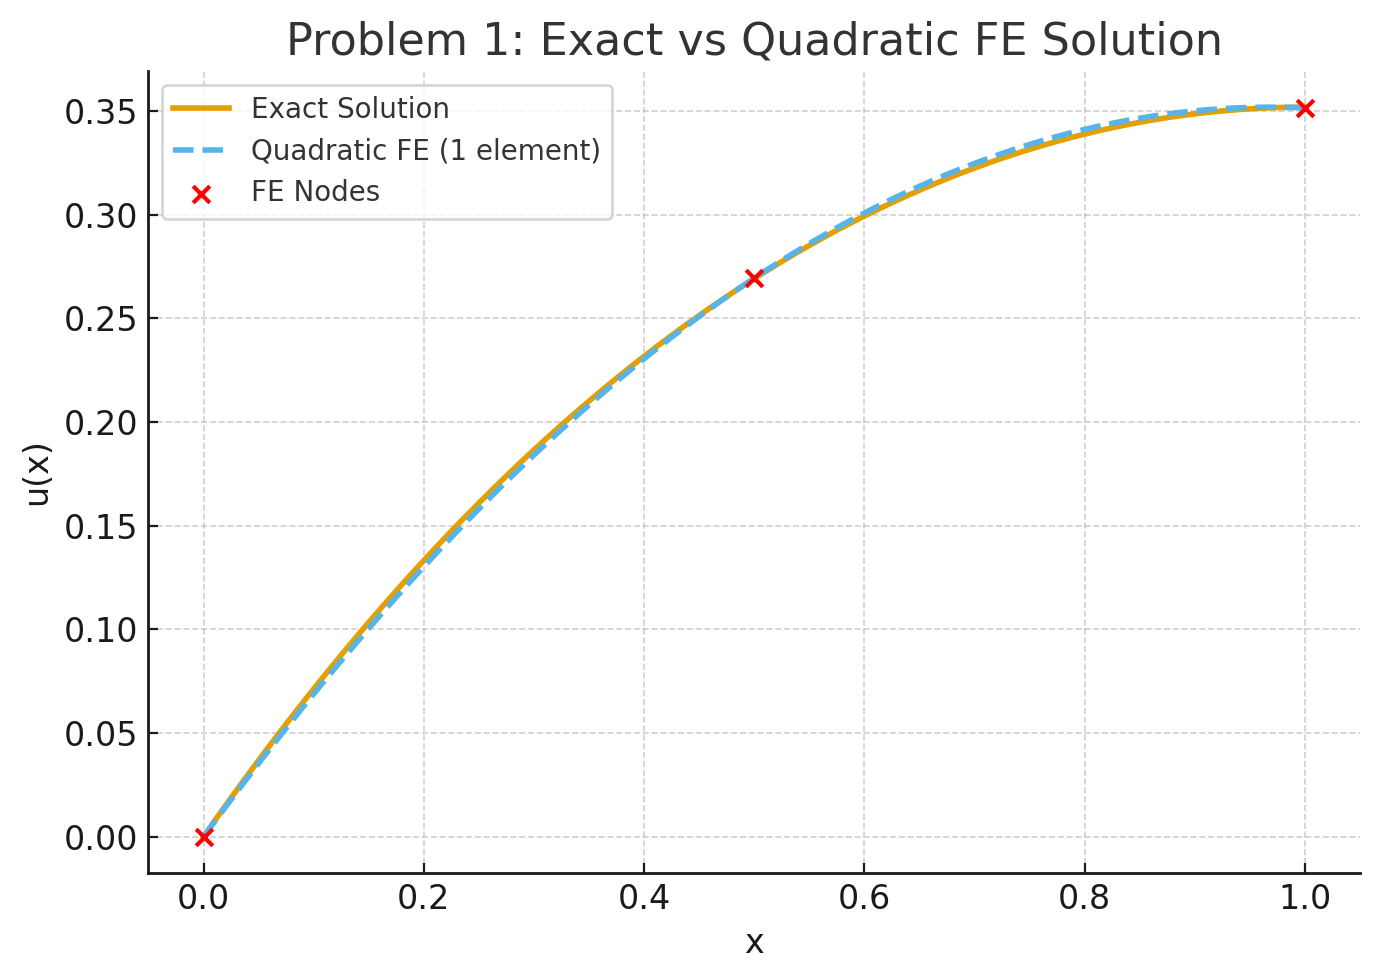
\includegraphics[width=0.7\linewidth]{hw3_prob1.png}
  \caption{Problem 1 exact field and quadratic finite element field.}
\end{figure}

\subsection*{Problem 2}
\paragraph{Exact field.}
For the source at $x=\tfrac12$ write two exponentials on the subintervals
\[
u(x)=
\begin{cases}
A_1 e^{x}+B_1 e^{-x}, & 0\le x\le \tfrac12,\\[2pt]
A_2 e^{x}+B_2 e^{-x}, & \tfrac12\le x\le 1.
\end{cases}
\]
Impose continuity at $x=\tfrac12$ and the jump in the derivative
\(
u'_R(\tfrac12)-u'_L(\tfrac12)=-1
\),
together with $u(0)=0$ and $u'(1)=1$, to determine $A_j,B_j$.

\paragraph{Two linear elements.}
Take two segments of length $\ell=\tfrac12$. The element matrix and vector for $-u''+u$ with unit right hand side over each element are
\[
K^{(e)}=\frac{1}{\ell}
\begin{bmatrix}
1&-1\\
-1&1
\end{bmatrix}
+\frac{\ell}{6}
\begin{bmatrix}
2&1\\
1&2
\end{bmatrix}.
\]
After assembly and inclusion of the unit point load at the middle node, one obtains
\[
\boldsymbol{F}=\begin{bmatrix}0\\1\\1\end{bmatrix},
\qquad
\boldsymbol{u}=
\begin{bmatrix}
0\\[2pt]
0.71409\\[2pt]
1.09380
\end{bmatrix}.
\]

\paragraph{Plots.}
\begin{figure}[H]
  \centering
  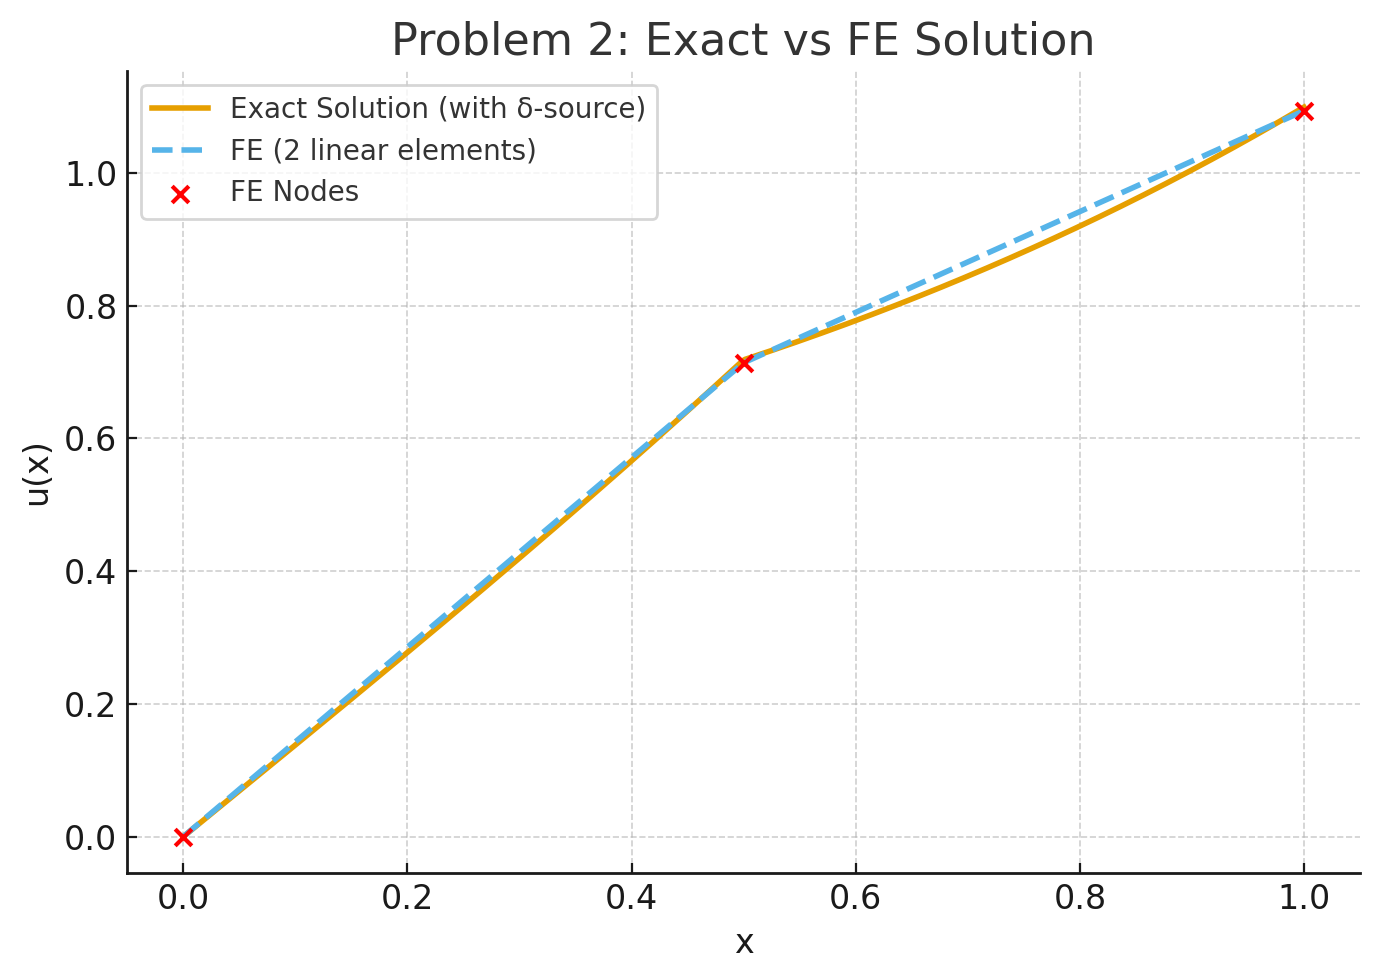
\includegraphics[width=0.7\linewidth]{hw3_prob2.png}
  \caption{Problem 2 exact field and linear finite element field.}
\end{figure}

\section*{Discussion}
The quadratic discretization in the first task tracks the curvature of the exact field with high accuracy on a single element. In the second task the pair of linear elements reproduces the correct change in slope at the source location and matches the analytic profile well away from the source.

\end{document}
